\item \textbf{{[}NYJC/PRELIM/9569/2021/P1/Q5{]} }

A school database has some data in the following table: 
\noindent \begin{center}
\begin{tabular}{|c|c|c|c|}
\hline 
\textbf{StudentID} & \textbf{Student Name } & \textbf{Class } & \textbf{Subjects}\tabularnewline
\hline 
1  & Wong Yong Ming  & 1917  & H2MATH, H2PHY, H2CHEM, H2ECON\tabularnewline
\hline 
2  & Vikram Singh  & 1911  & H2MATH, H2CHEM, H2ECON,H1GEOG\tabularnewline
\hline 
3  & Muhd Bashir bin Ramdan  & 1911 & H2MATH, H2CHEM, H2ECON, H1ELIT\tabularnewline
\hline 
\end{tabular} 
\par\end{center}
\begin{enumerate}
\item {}
\begin{enumerate}
\item State and explain if the above table is in third normal form (3NF).
\hfill{}{[}4{]}
\item Describe two advantages that normalised data has over redundant data.
\hfill{}{[}2{]}
\end{enumerate}
\end{enumerate}
In an effort to improve the school database, the IT administrator
came up with an ER diagram. Part of the full ER diagram is as shown. 
\begin{center}
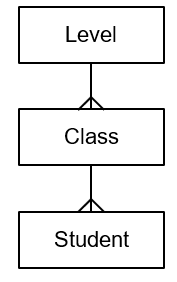
\includegraphics[width=0.15\paperwidth]{C:/Users/Admin/Desktop/Github/question_bank/LyX/static/img/9569-NYJC-2021-P1-Q5}
\par\end{center}

Each of the three entities in the ER diagram has a name attribute. 
\begin{enumerate}
\item[(b)] {}  
\begin{enumerate}
\item Write table descriptions to implement the above ER diagram. \hfill{}{[}5{]}
\item Write an SQL query to retrieve only the student name and class name
for all students in the level \texttt{JC2}. \hfill{}{[}3{]}
\end{enumerate}
\end{enumerate}
A fast-growing startup is writing code to provide a new service. The
user needs have not yet been fully determined, and the data schema
is likely to undergo further changes before being finalised. 
\begin{enumerate}
\item[(c)]  {}
\begin{enumerate}
\item Suggest if SQL or NoSQL is more suitable for the needs of this startup.
Give \textbf{two} reasons to support your answer.\hfill{} {[}4{]}
\item Describe \textbf{two} challenges the startup will face in using NoSQL
databases.\hfill{} {[}2{]}
\end{enumerate}
\item[(d)]  The startup is concerned that a hardware failure may wipe out critical
data and leave them unable to continue operating. 

Suggest what the startup should do to \textbf{ensure} that they are
safe against data loss in such a scenario.\hfill{} {[}4{]}
\end{enumerate}